\section{Bridging between IB and CB in Java}\label{sec:imp}


%\footnote{ Rewriting libraries and
%  application in this language/model would result in more reusable
%  libraries, but it would be a taunting task.}
Creating a new language or a language extension would be an
elegant way to illustrate the point of IB. However,
significant amounts of engineering would be needed to build a practical
language, and to achieve a similar level of integration and tool support
as Java. To have an approach that can both illustrate IB
programming and be practical, we have instead implemented 
\mixin as an annotation over Java 8, and a \emph{compilation agent}.
That is, the Classless Java style of programming
is supported by a Java 8 library.

Disciplined use of Classless Java (that is avoiding class
declarations as done in Section~\ref{sec:ep}), illustrates what \emph{pure} IB is like.
However, using \mixin, CB and IB programming can be mixed together, 
harvesting the practical convenience of using existing Java libraries, the full
Java language, and IDE's support.
The key to our implementation is the use of compilation agents, which
 allows us to rewrite the Java AST just
before compilation. We discuss advantages and limitations of our approach.

\subsection{Compilation Agents}
Java supports compilation agents, where Java libraries can interact with the Java compilation process,
acting as a man in the middle between the
generation of the abstract syntax tree and the Java bytecode.

This process is facilitated by frameworks like Lombok~\cite{lombok}:
a Java library that aims at removing (or
reducing) Java boilerplate code via
annotations. \mixin was created using Lombok.
Figure~\ref{fig:lombok}~\cite{neildo2011blog} illustrates the flow of
the \mixin annotation.
First java source code is parsed into an abstract syntax tree (AST).
The AST is then captured by Lombok:
each annotated node is passed to
the corresponding (Eclipse or Javac) handler. The handler is
free to modify the information of the annotated node, or even inject new nodes (like methods, inner classes,
etc). Finally, the Java compiler works on the modified AST to generate bytecode.
%Note how during the compilation,
%no source code is changed, and no new source/temporary files are created.

 
%There are a number of annotations provided by the
%original Lombok, including \Q:@Getter:, \Q:@Setter:,
%\Q:@ToString: for generating getters, setters and \QM{toString}
%methods, respectively.  Furthermore, Lombok provides a number of
%interfaces for users to create custom transformations, as extensions
%to the original framework.
%A transformation is based on a handler, which acts on the AST for the
%annotated node and returns a modified AST for analysis and
%generation afterwards. Such a handler can either be a Javac handler or
%an Eclipse handler.

\begin{figure}[t]
\saveSpaceFig
\centering
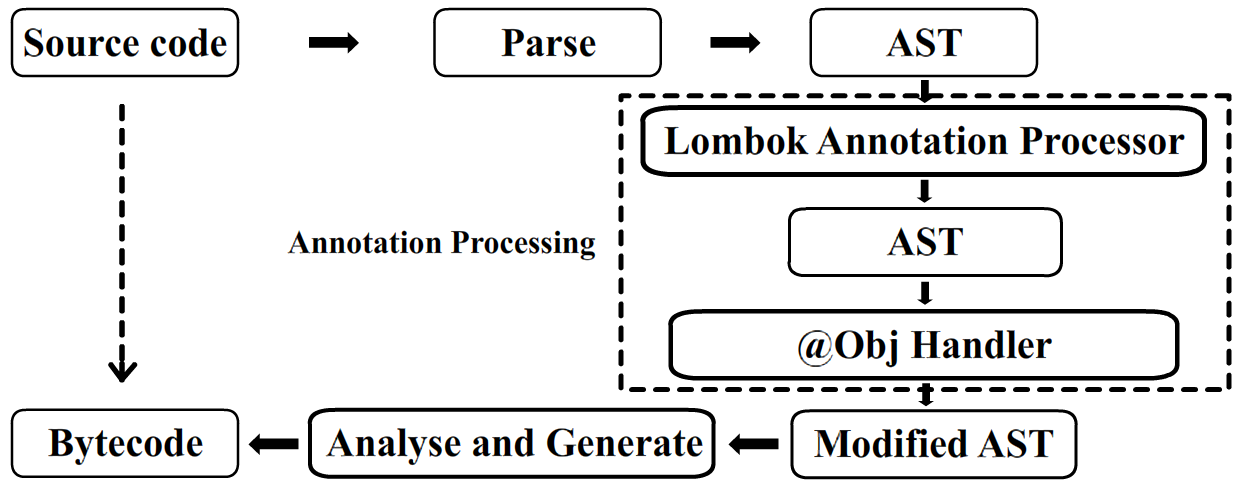
\includegraphics[width=3in]{pdfs/lombok3.png}
\caption{The flow chart of \mixin annotation processing.
}
\label{fig:lombok}
\saveSpaceFig
\end{figure}


\paragraph{Advantages of Lombok}
The Lombok compilation agent has advantages with respect to alternatives like
pre-processors, or other Java annotation processors.
Lombok offers in Java an expressive power similar to that of Scala/Lisp macros;
except of course, for the syntactic convenience of quote/unquote templating.


\paragraph{Direct modification of the AST:}
Lombok alters the generation process of the class files,
by directly modifying the AST. Neither the source code is modified nor
new Java files are generated. Moreover, and probably more importantly,
Lombok supports generation of code \emph{inside} a class/interface,
which conventional Java annotation processors do not support. For
example, the standard \texttt{javax.annotation} processor, which is part of the
Java platform, only allows generation of \emph{new code}, and the
new code has to be written in \emph{new files}. Modification and/or
reinterpretation of existing code is not supported.

\paragraph{Modularity}
While general preprocessing acts across module boundaries, compilation
agents act modularly on each class/compilation unit. It makes sense to
apply the transformations to one class/interface at a time, and only to
annotated classes/interfaces. This allows library code to be reused
without the need of being reprocessed and recompiled, making our
approach 100\% compatible with existing Java libraries, which can be
used and extended normally. Of course, Java libraries can also receive
and use instances of object interfaces as normal objects.

\begin{figure*}[t]
\saveSpaceFig
\saveSpaceFig
\centering
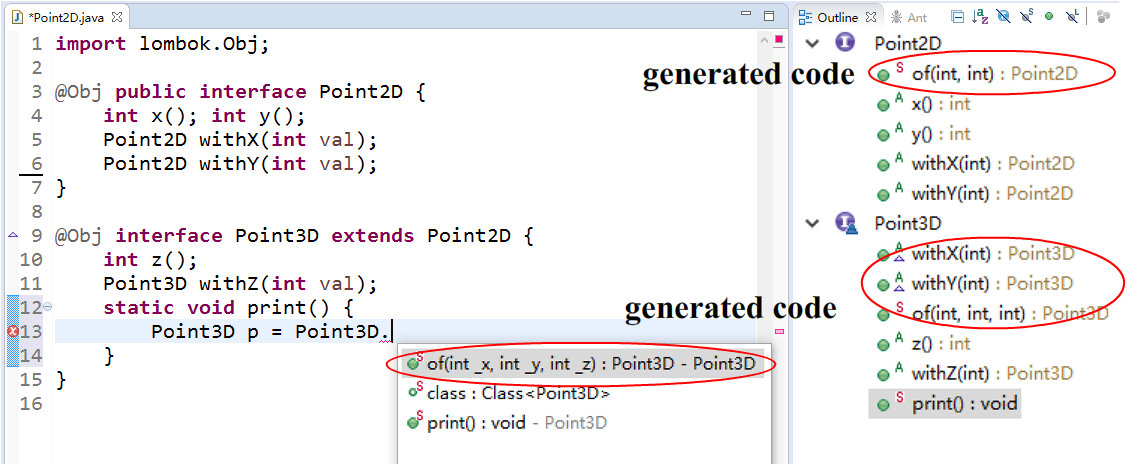
\includegraphics[width=6in]{pdfs/screenshot4.png}
\caption{Generated methods shown in the Outline window of Eclipse and auto-completion.}
\label{fig:screenshot}
\saveSpaceFig
\end{figure*}

\paragraph{Tool support}
Features written in Lombok integrate and are supported directly in the
language, and are often also supported by (most) tools.  For example in Eclipse, the processing is
performed transparently and the information of the interface from
compilation is captured in the ``Outline'' window.
This includes all
the methods inside the interface as well as the generated ones.
In Figure~\ref{fig:screenshot},
\mixin generates an \Q@of@ method in \Q@Point2D@, and \Q@of@, \Q@withX@, \Q@withY@ methods in \Q@Point3D@.
These methods are also visible to users, showing their types and modifiers in Outline window.
Moreover, as a useful IDE feature, the auto-completion also works for these newly generated methods.

\paragraph{Clarity against obfuscation:}
Preprocessors bring great power, which can easily be misused producing
code particularly hard to understand. Thus code quality and maintainability are reduced.
Compilation agents start from Java syntax, but they can reinterpret it.
Preserving the syntax avoids syntactic conflicts, and allows many
tools to work transparently.

\subsection{\mixin AST Reinterpretation}

Of course, careless reinterpretation of the AST could still be
surprising for badly designed rewritings.  \mixin reinterprets
the syntax with the sole goal of \emph{enhancing and completing code}:
we satisfy the behaviour of abstract methods; add method
implementations; and refine return types.  We consider this to be
quite easy to follow and reason about, since it is similar to what
happens in normal inheritance.  Refactoring operations like renaming
and moving should work transparently in conjunction with our
annotation, since they rely on the overall type structure of the
class, which we do not arbitrarily modify but just complete.

Thus, in addition to the advantages of Lombok, Classless Java offers
some more advantages with respect to arbitrary (Compilation agent driven) AST rewriting.

%\marco{The section No reuse of the type system
%is controversial.
%We do need to repeat the type checking, plus we aim to make untypable stuff well typed
%(for example anyone using the of method would not be well typed before).}
%\item \textbf{No reuse of the type system.}
%As we mentioned above, badly designed rewritings can arise from the great power of Lombok. A simple piece of source code
%\begin{lstlisting}
%interface M { int m(); }
%\end{lstlisting}
%can be reinterpreted as
%\begin{lstlisting}
%interface M { void m(String s); }
%\end{lstlisting}
%in which case the type of method \Q@m@ is changed. Our \mixin annotation does not introduce this kind of rewritings,
%and hence the type system is reused. Moreover, Lombok can also modify unbounded types, which is easy to understand,
%for instance, the following code
%\begin{lstlisting}
%interface M { T m(); } // T is unbounded
%\end{lstlisting}
%is transformed into
%\begin{lstlisting}
%interface M { int m(); } // No error message
%\end{lstlisting}
%in which case the user will see the unbounded type in source code, but without error message from the compilation, since
%Lombok has modified the return type of \Q@m@. However, our \mixin annotation can still keep such errors and warnings.


%\item \textbf{Lack of reuse.}  %not sure here... I think most preprocessors support decent reuse, even the C one
%Reusability is yet another concern in using preprocessors.
% In Lombok, implementations of features are
%encapsulated in various annotation handlers,
% in which case some behaviours are allowed to reuse the code by invoking methods
%in other handlers, where tedious replicated code is avoided.



\paragraph{Syntax and type errors}:
Some preprocessors (like the C one) can produce syntactically invalid code.
Lombok ensures only syntactically valid code is produced. %; however, type errors can appear.
Classless Java additionally guarantees that no type errors are introduced
in generated code and client code. We discuss these two guarantees in
more detail next:

\begin{itemize}

\item{\bf Self coherence}: The generated code itself is well-typed. That is,
  type errors are not present in code the user has not written (for
  example \texttt{of} methods in Figure~\ref{fig:screenshot}).
In our case it means that either \mixin{} produces (in a controlled way) an
understandable error, or the interface can be successfully annotated and the generated code is well-typed.

\item{\bf Client coherence}: All the client code (for example method calls)
  that is well-typed before code generation is also well-typed after the generation.
The annotation just adds more behaviour without removing any functionality.

\end{itemize}

\paragraph{Heir coherence}: Another form of guarantee that could be
useful in AST rewriting is heir coherence. That is, interfaces
(and in general classes) inheriting the instrumented code are
well-typed if they were well-typed without the instrumentation.
In a strict sense, our rewriting \emph{does not} guarantee heir coherence.  The reason
is that this would forbid adding any (default or abstract) method to
the annotated interfaces, or even doing type refinement. Indeed consider
the following:

\begin{lstlisting}
interface A { int x(); A withX(int x); }
@Obj interface B extends A {}
interface C extends B { A withX(int x); }
\end{lstlisting}

\noindent This code is correct before the translation, but \mixin would  generate in \Q@B@  a method ``\Q@B withX(int x);@''.
This would break \Q@C@.
Similarly, an expression of the form ``\Q@new B(){.. A withX(int x){..}}@''
would be correct before translation, but ill-typed after the translation.

Our automatic type refinement is a useful and convenient feature, but
not transparent to the heirs of the annotated interface.  They need to
be aware of the annotation semantics and provide the right type while
refining methods. To support heir coherence, we would need
to give up automatic type refinement, which is an essential part of IB programming.
However, the reader should note that Java libraries almost always break heir
coherence during evolution and still claim backward compatibility (false in
theory but statistically true in practice). In practice, adding any method to any
non final class of a Java library is enough to break heir
coherence.  We think return type refinement breaks heir coherence ``less" than normal library evolution, and
if no automatic type-refinements are needed, then \mixin can claim a
form of heir coherence.

Section~\ref{sec:translation} provide a formal definition for our
safety claims.

\subsection{Limitations}
Our prototype implementation has certain limitations:
\begin{itemize}
\item Eclipse has its own compiler (ejc), alternative to javac.
  Lombok allows writing handlers for either javac or ejc.
  At this stage our implementation only realizes the Eclipse handler and our
  experiments are all conducted in Eclipse. The implementation for
  the \texttt{javac} handler is still missing.
\item The current implementation supports generics in a simplified manner: 
type parameters can be used but the generic
method typing is neither formalized in this paper nor explicitly checked by our 
implementation, but simply  delegated to the Java compiler.
\item 
Lombok offers only limited/experimental support for separate compilation, that is
to access information of code defined in different files.
In the same spirit, we have a mature \mixin annotation, that
does not support separate compilation yet: it requires that all
  related interfaces have to appear in a single Java file.
Reusing the logic inside the yet experimental Lombok annotation \lstinline{@Delegate},
we also offer a less polished annotation supporting
separate compilation for files in the same package.
%  has the same behavior as \mixin. A limitation is
%  that users need to put references to the super types
% of the annotated type together with the annotation, for instance,
%  \lstinline{@Delegate(types = Point2D.class)}.
%   Another limitation is the methods generated by \lstinline{@Delegate} will
%  not be visible in the Outline window, but they can still be auto-completed in Eclipse.
\end{itemize}


%\paragraph{Lombok does language tuning}
%We consider Lombok to be the most developed example of language
%tuning.  While the authors of Lombok do not introduce a specific term
%for what they are doing, their slogan \emph{``Spice up your java''}
%seems to be in line with the philosophy of language tuning. Some
%other examples of language tuning in Lombok include the \Q@val@ type,
%similar to \Q@auto@ in C\# or C++04.  Another library doing language
%tuning is CoFoJa~\cite{cofoja}, where annotations are used to insert
%pre-post conditions in generated bytecode.

